%%% template.tex
%%%
%%% This LaTeX source document can be used as the basis for your technical
%%% paper or abstract. Intentionally stripped of annotation, the parameters
%%% and commands should be adjusted for your particular paper - title, 
%%% author, article DOI, etc.
%%% The accompanying ``template.annotated.tex'' provides copious annotation
%%% for the commands and parameters found in the source document. (The code
%%% is identical in ``template.tex'' and ``template.annotated.tex.'')

\documentclass[conference]{acmsiggraph}

\usepackage{authblk}
\usepackage[]{algorithm2e}

\TOGonlineid{45678}
\TOGvolume{0}
\TOGnumber{0}
\TOGarticleDOI{1111111.2222222}
\TOGprojectURL{}
\TOGvideoURL{}
\TOGdataURL{}
\TOGcodeURL{}

\title{Performance Driven Redundancy Optimization of Data Layouts for Walkthrough Applications}

%\author[1]{Zachary DeStefano\thanks{zdestefa@uci.edu}}
%\author[1]{Shan Jiang\thanks{sjiang1714@gmail.com}}
%\author[1]{Gopi Meenakshisundaram\thanks{gopi.meenakshisundaram@gmail.com}}
%\author[2]{Sung-Eui Yoon\thanks{toinsert}}
%\pdfauthor{Zachary DeStefano,Shan Jiang,Gopi Meenakshisundaram,Sung-Eui Yoon}
\pdfauthor{}
\author{}
%\affil[1]{University of California, Irvine}
%\affil[2]{KAIST}

\keywords{Data Layout Problem, Out-Of-Core Rendering, Cache Oblivious Mesh Layout, Redundant Data Layout, Walkthrough Application}

\begin{document}

%% \teaser{
%%   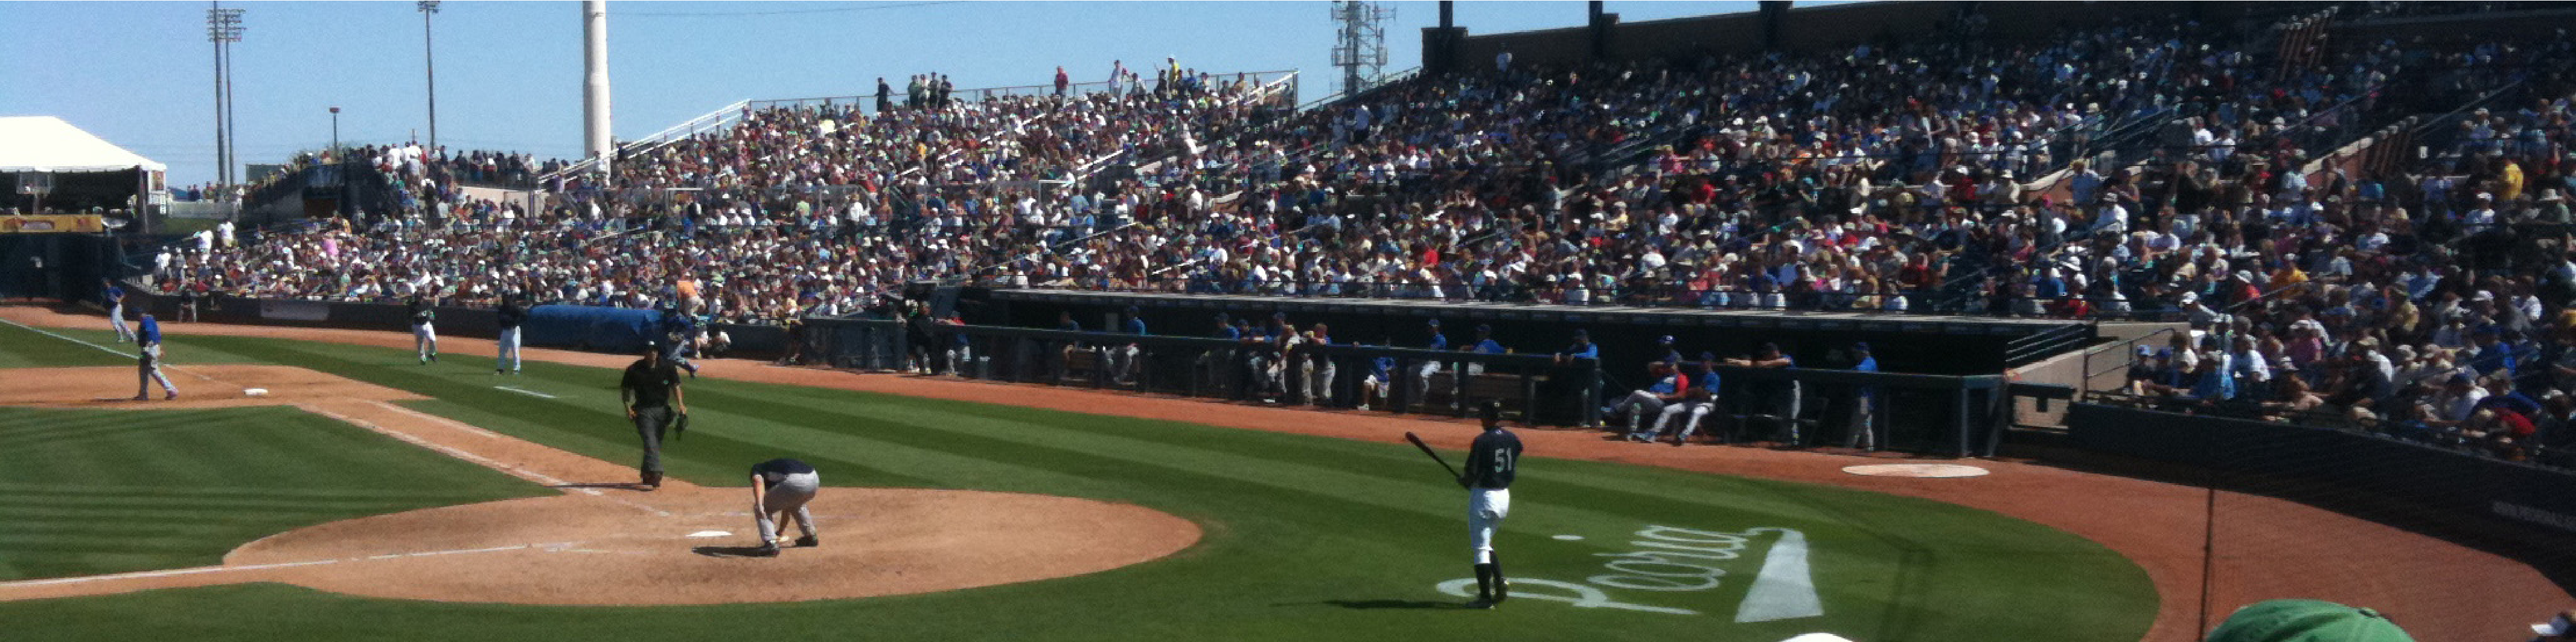
\includegraphics[height=1.5in]{images/sampleteaser}
%%   \caption{Spring Training 2009, Peoria, AZ.}
%% }

\maketitle

\section{Analysis and Comparisons over Prior methods}

In the algorithm, we make a list of data units that will reduce seek time by just moving them. We perform these moves first before doing any copying. This initial step will produce a better solution than proposed by \cite{cacheobliviouslayout} without adding extra units. This is because our algorithm will consider cases where data units are close to each other but in hierarchically different blocks with  the cache oblivious layout. To show this, consider a case where we have two access requirements of 5 data units each. Figure \ref{YoonImprovement} shows an example of that kind of layout. In the middle of that figure is the result of using the cache oblivious layout. Because hierarchically it would arrange the units in each block and then arrange the blocks, it does not detect that the units with the black access requirement can be grouped together. When our algorithm is run, it would find that it can shorten the black access requirements without adding redundancy so it would do that first, as shown in the bottom of that figure.

\begin{figure}[ht]
\centering
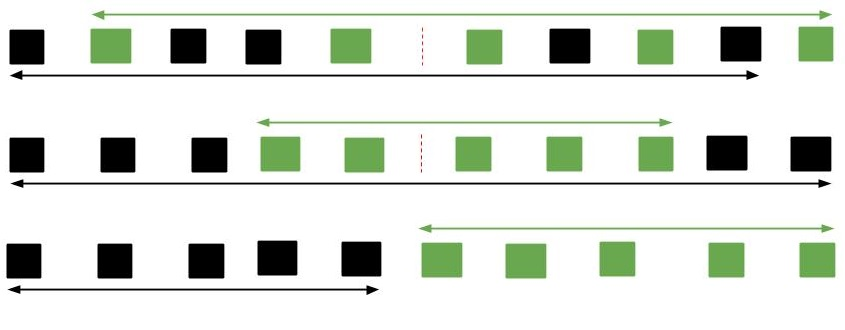
\includegraphics[width=3in]{ImprovementOverYoon.jpg}
\caption{Example of two access requirements of 5 data units each. The red line represents the boundary between blocks in the cache oblivious layout hierarchy. The original layout (top), cache-oblvious layout (middle), as well as the layout after running our algorithm (bottom) is shown.}
\label{YoonImprovement}
\end{figure}

Existing algorithms for the data layout problem do not consider redundancy. Even if we find a polynomial time algorithm that solves the data layout problem, we can actually achieve a seek time better than the optimal one without redundancy. We have such an example with figure \ref{fig:startingProb}. As can be seen in the figure, the total seek time is 11 units originally. Without redundancy, the seek time is reduced to 9 units, as found through a brute-force search. With redundancy, the total seek time is the minimum required which is 8 units. While a reduction from 9 to 8 units may not seem dramatic, when this result is scaled up to the hundreds of millions, this makes a big difference in seek time, which we saw in practice.\\

\begin{figure}[ht]
\centering
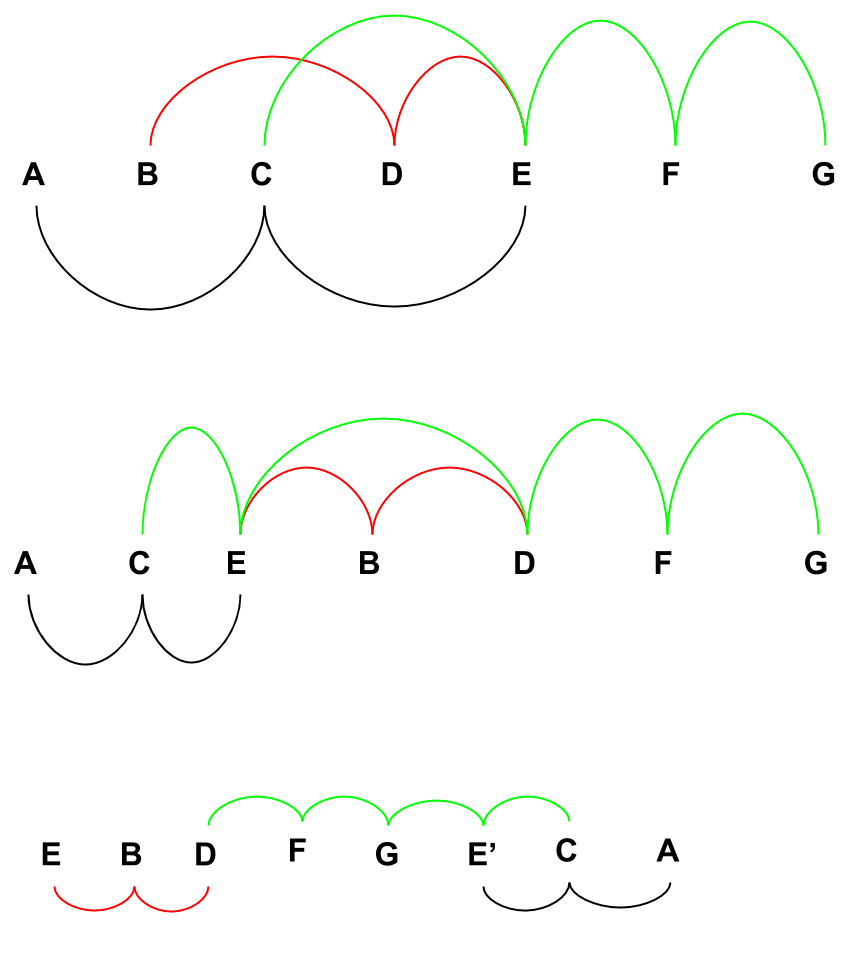
\includegraphics[width=3in]{examplePic.png}
\caption{Data Units with varying access requirements (top) as well as its optimal layout without redundancy (middle) and its optimal layout with redundancy (bottom)}
\label{fig:startingProb}
\end{figure}

\section{Conclusion and Future Work}

We have shown that we have an algorithm with an efficient running time and storage space for the Data Layout Problem. It achieves significant results analytically and experimentally. When walking through an extremely detailed 3D model, this algorithm can be used to ensure that the performance will not suffer. If we give the algorithm the proper access requirements with this 3D model, then the performance will be even better.\\
\\
This leads to a logical extension of this work. Since we have a good algorithm that takes over once we know the access requirements, we should figure out how to ensure there are good access requirements to begin with. One idea on how to ensure this is to check the usage history of an application and group data units together if they are accessed together with high probability. This could even be done dynamically in the sense that after a certain amount of usage and repeating on a regular basis, you recompute the optimal access requirements and then use that to recompute the optimal layout. 

\bibliographystyle{acmsiggraph}
\bibliography{finalPaperRefs}

\end{document}
